\documentclass{if-beamer}

% --------------------------------------------------- %
%                  Presentation info	              %
% --------------------------------------------------- %
\title[Lecture 16]{Lecture 16}
\subtitle{Optimization: Parabolic Interpolation}
\author{Ashley Gannon}
\date{ISC3313 Fall 2021}
\logo{
\includegraphics[scale=0.08]{figures/FSULogo.png}
}
\subject{Presentation subject}

% --------------------------------------------------- %
%                    Title + Schedule                 %
% --------------------------------------------------- %
\begin{document}

\begin{frame}
  \titlepage
\end{frame}
% --------------------------------------------------- %
%                      Presentation                   %
% --------------------------------------------------- %
\section{Parabolic Interpolation}

\begin{frame}
	\frametitle{Parabolic Interpolation}
	Parabolic interpolation takes advantage of the fact that a second-order polynomial often
	provides a good approximation to the shape of $f(x)$ near an optimum.
	\begin{figure}
		\centering
		\includegraphics[width = .5\textwidth]{figures/para1}
	\end{figure} 
\end{frame}

\begin{frame}
	\frametitle{Parabolic Interpolation}
	Parabolic interpolation takes advantage of the fact that a second-order polynomial often
	provides a good approximation to the shape of $f(x)$ near an optimum.
	\begin{figure}
		\centering
		\includegraphics[width = .5\textwidth]{figures/para2}
	\end{figure} 
	In this method, we choose three points that jointly bracket an optimum. 
\end{frame}

\begin{frame}
	\frametitle{Parabolic Interpolation}
	Parabolic interpolation takes advantage of the fact that a second-order polynomial often
	provides a good approximation to the shape of $f(x)$ near an optimum.
	\begin{figure}
		\centering
		\includegraphics[width = .5\textwidth]{figures/para3}
	\end{figure} 
	In this method, we choose three points that jointly bracket an optimum. If $x_2 < x_1 \textrm{ and } x_3$ or $x_2 > x_1 \textrm{ and } x_3$, we can fit a parabola to the points using Lagrange interpolation. 
\end{frame}

\begin{frame}[t]
	\frametitle{Parabolic Interpolation}
	$q(x)$ is the parabolic function based on the three points chosen:
	$$q(x) = f(x_1)\frac{(x_4-x_2)(x_4-x_3)}{(x_1-x_2)(x_1-x_3)}+f(x_2)\frac{(x_4-x_3)(x_4-x_1)}{(x_2-x_3)(x_2-x_1)}+f(x_3)\frac{(x_4-x_1)(x_4-x_2)}{(x_3-x_1)(x_3-x_2)} $$
\end{frame}

\begin{frame}[t]
	\frametitle{Parabolic Interpolation}
	$q(x)$ is the parabolic function based on the three points chosen:
	$$q(x) = f(x_1)\frac{(x_4-x_2)(x_4-x_3)}{(x_1-x_2)(x_1-x_3)}+f(x_2)\frac{(x_4-x_3)(x_4-x_1)}{(x_2-x_3)(x_2-x_1)}+f(x_3)\frac{(x_4-x_1)(x_4-x_2)}{(x_3-x_1)(x_3-x_2)} $$
	To find the optimum of this function, we need to take it's derivative and set it to 0.
	\begin{align*}
	q'(x) = & f(x_1)\frac{(x_4-x_2)+(x_4-x_3)}{(x_1-x_2)(x_1-x_3)}+f(x_2)\frac{(x_4-x_3)+(x_4-x_1)}{(x_2-x_3)(x_2-x_1)}\\
	&+f(x_3)\frac{(x_4-x_1)+(x_4-x_2)}{(x_3-x_1)(x_3-x_2)} = 0
	\end{align*}
\end{frame}

\begin{frame}[t]
	\frametitle{Parabolic Interpolation}
	$q(x)$ is the parabolic function based on the three points chosen:
	$$q(x) = f(x_1)\frac{(x_4-x_2)(x_4-x_3)}{(x_1-x_2)(x_1-x_3)}+f(x_2)\frac{(x_4-x_3)(x_4-x_1)}{(x_2-x_3)(x_2-x_1)}+f(x_3)\frac{(x_4-x_1)(x_4-x_2)}{(x_3-x_1)(x_3-x_2)} $$
	To find the optimum of this function, we need to take it's derivative and set it to 0.
	\begin{align*}
		q'(x) = & f(x_1)\frac{(x_4-x_2)+(x_4-x_3)}{(x_1-x_2)(x_1-x_3)}+f(x_2)\frac{(x_4-x_3)+(x_4-x_1)}{(x_2-x_3)(x_2-x_1)}\\
		&+f(x_3)\frac{(x_4-x_1)+(x_4-x_2)}{(x_3-x_1)(x_3-x_2)} = 0
	\end{align*}
	Now we need to solve for our unknown point, $x_4$
	$$x_4 = x_2 - \frac{1}{2}\frac{(x_2-x_1)^2[f(x_2)-f(x_3)]-(x_2-x_3)^2[f(x_2)-f(x_1)]}{(x_2-x_1)[f(x_2)-f(x_3)]-(x_2-x_3)[f(x_2)-f(x_1)]}$$
	where $x_1$, $x_2$, and $x_3$ are the initial guesses, and $x_4$ is the value of $x$ that corresponds to the
	optimum value of the parabolic fit to the guesses.
\end{frame}

\begin{frame}
	\frametitle{Parabolic Interpolation Example}
	Let's revisit our example from the previous lectures
	$$f(x) = \frac{x^2}{10}-2sin(x)$$
    Remembering our plot:
	\begin{figure}
		\centering
		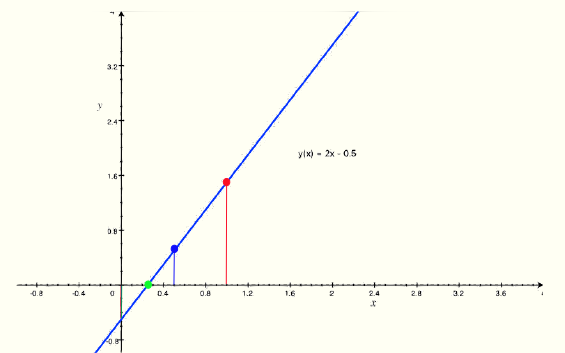
\includegraphics[width=.65\textwidth]{figures/plot}
	\end{figure}
And let's start with initial guesses of $x_1 = 0$, $x_2 = 1$, and $x_3 = 4$.
\end{frame}

\begin{frame}[t]
\frametitle{Parabolic Interpolation Example}
The first thing we'll do is calculate $x_4$.
$$ x_4 = 1-\frac{1}{2}\frac{(1-0)^2[-1.5829-3.1136]-(1-4)^2[-1.5829-0]}{(1-0)[-1.5829-3.1136]-(1-4)[-1.5829-0]}=1.5055$$	
\end{frame}

\begin{frame}[t]
	\frametitle{Parabolic Interpolation Example}
	The first thing we'll do is calculate $x_4$.
	$$ x_4 = 1-\frac{1}{2}\frac{(1-0)^2[-1.5829-3.1136]-(1-4)^2[-1.5829-0]}{(1-0)[-1.5829-3.1136]-(1-4)[-1.5829-0]}=1.5055$$	
	Next, a strategy similar to the golden-section search can be employed to determine
	which point should be discarded.\\
	\begin{minipage}{0.5\textwidth}
		\begin{align*}
			f(x_1) &= 0\\
			\mathbf{f(x_2)} &= \mathbf{-1.5829}\\
			f(x_3) &= 3.1136\\
			\mathbf{f(x_4)} &= \mathbf{-1.7691}\\
		\end{align*}
	\end{minipage}
	\begin{minipage}{0.5\textwidth}
		\begin{figure}
			\centering
			\includegraphics[width=\textwidth]{figures/plot2}
		\end{figure}
	\end{minipage}
\end{frame}

\begin{frame}[t]
	\frametitle{Parabolic Interpolation Example}
	The first thing we'll do is calculate $x_4$.
	$$ x_4 = 1-\frac{1}{2}\frac{(1-0)^2[-1.5829-3.1136]-(1-4)^2[-1.5829-0]}{(1-0)[-1.5829-3.1136]-(1-4)[-1.5829-0]}=1.5055$$	
	Next, a strategy similar to the golden-section search can be employed to determine
	which point should be discarded.\\
	\begin{minipage}{0.5\textwidth}
		\begin{align*}
			f(x_1) &= 0\\
			\mathbf{f(x_2)} &= \mathbf{-1.5829}\\
			f(x_3) &= 3.1136\\
			\mathbf{f(x_4)} &= \mathbf{-1.7691}
		\end{align*}
	Since $f(x_2)>f(x_4)$
	\begin{align*}
		x_1 &\leftarrow x_2\\
		x_2 &\leftarrow x_4\\
		x_3 &= x_3\\
	\end{align*}
	\end{minipage}
	\begin{minipage}{0.5\textwidth}
		\begin{figure}
			\centering
			\includegraphics[width=\textwidth]{figures/plot2}
		\end{figure}
	\end{minipage}
\end{frame}


\begin{frame}[t]
	\frametitle{Parabolic Interpolation Example}
	The first thing we'll do is calculate $x_4$.
	$$ x_4 = 1-\frac{1}{2}\frac{(1-0)^2[-1.5829-3.1136]-(1-4)^2[-1.5829-0]}{(1-0)[-1.5829-3.1136]-(1-4)[-1.5829-0]}=1.5055$$	
	Next, a strategy similar to the golden-section search can be employed to determine
	which point should be discarded.\\
	\begin{minipage}{0.5\textwidth}
		\begin{align*}
			f(x_1) &= 0\\
			\mathbf{f(x_2)} &= \mathbf{-1.5829}\\
			f(x_3) &= 3.1136\\
			\mathbf{f(x_4)} &= \mathbf{-1.7691}
		\end{align*}
		Since $f(x_2)>f(x_4)$
		\begin{align*}
			x_1 &\leftarrow x_2\\
			x_2 &\leftarrow x_4\\
			x_3 &= x_3\\
		\end{align*}
	\end{minipage}
	\begin{minipage}{0.5\textwidth}
		\begin{figure}
			\centering
			\includegraphics[width=\textwidth]{figures/plot3}
		\end{figure}
	\end{minipage}
\end{frame}

\begin{frame}[t]
	\frametitle{Parabolic Interpolation Example}
	Now we need to recalculate $x_4$.
	\begin{align*}
	x_4 &= 1.5055-\frac{1}{2}\frac{(1.5055-1)^2[-1.7691-3.1136]-(1.5055-4)^2[-1.7691-(-1.5829)]}{(1.5055-1)[-1.7691-3.1136]-(1.5055-4)[-1.7691-(-1.5829)]}\\
	&=1.4903\\
\end{align*}	
\end{frame}

\begin{frame}[t]
	\frametitle{Parabolic Interpolation Example}
	Now we need to recalculate $x_4$.
	\begin{align*}
	x_4 &= 1.5055-\frac{1}{2}\frac{(1.5055-1)^2[-1.7691-3.1136]-(1.5055-4)^2[-1.7691-(-1.5829)]}{(1.5055-1)[-1.7691-3.1136]-(1.5055-4)[-1.7691-(-1.5829)]}\\
	&=1.4903\\
\end{align*}	
	And then determine which point should be discarded.\\
	\begin{minipage}{0.5\textwidth}
		\begin{align*}
			f(x_1) &= -1.5829\\
			\mathbf{f(x_2)} &= \mathbf{-1.7691}\\
			f(x_3) &= 3.1136\\
			\mathbf{f(x_4)} &= \mathbf{-1.7714}\\
		\end{align*}
	\end{minipage}
	\begin{minipage}{0.5\textwidth}
		\begin{figure}
			\centering
			\includegraphics[width=\textwidth]{figures/plot4}
		\end{figure}
	\end{minipage}
\end{frame}

\begin{frame}[t]
	\frametitle{Parabolic Interpolation Example}
	Now we need to recalculate $x_4$.
	\begin{align*}
		 x_4 &= 1.5055-\frac{1}{2}\frac{(1.5055-1)^2[-1.7691-3.1136]-(1.5055-4)^2[-1.7691-(-1.5829)]}{(1.5055-1)[-1.7691-3.1136]-(1.5055-4)[-1.7691-(-1.5829)]}\\
		 &=1.4903
	\end{align*}	
	And then determine which point should be discarded.\\
	\begin{minipage}{0.5\textwidth}
		\begin{align*}
			f(x_1) &= -1.5829\\
			\mathbf{f(x_2)} &= \mathbf{-1.7691}\\
			f(x_3) &= 3.1136\\
			\mathbf{f(x_4)} &= \mathbf{-1.7714}
		\end{align*}
		Since $f(x_2) > f(x_4)$
		\begin{align*}
		x_1 &= x_1\\
		x_3 &\leftarrow x_2\\
		x_2 &\leftarrow x_4\\
		\end{align*}
	\end{minipage}
	\begin{minipage}{0.5\textwidth}
		\begin{figure}
			\centering
			\includegraphics[width=.9\textwidth]{figures/plot4}
		\end{figure}
	\end{minipage}
\end{frame}
%
%\begin{frame}[t]
%	\frametitle{Parabolic Interpolation Example}
%	Now we need to recalculate $x_4$.
%	\begin{align*}
%		x_4 &= 1.5055-\frac{1}{2}\frac{(1.5055-1)^2[-1.7691-3.1136]-(1.5055-4)^2[-1.7691-(-1.5829)]}{(1.5055-1)[-1.7691-3.1136]-(1.5055-4)[-1.7691-(-1.5829)]}\\
%		&=1.4903
%	\end{align*}	
%	And then determine which point should be discarded.\\
%	\begin{minipage}{0.5\textwidth}
%		\begin{align*}
%			f(x_1) &= -1.5829\\
%			f(x_2) &= -1.7691\\
%			f(x_3) &= 3.1136\\
%			f(x_4) &= -1.7714
%		\end{align*}
%		Since $x_2 > x_4$
%		\begin{align*}
%			x_1 &= x_1\\
%			x_3 &\leftarrow x_2\\
%			x_2 &\leftarrow x_4\\
%		\end{align*}
%	\end{minipage}
%	\begin{minipage}{0.5\textwidth}
%		\begin{figure}
%			\centering
%			\includegraphics[width=.9\textwidth]{figures/plot5}
%		\end{figure}
%	\end{minipage}
%	Keep iterating until $error = |\frac{x_4-x_4_{old}}{x_4}| < tol$
%\end{frame}

\begin{frame}
	\frametitle{Parabolic Interpolation Pseudocode}
	
	\texttt{declare tol, x4old}\\
	\texttt{declare/define error}\\\vspace{10pt}
	\texttt{define/declare $x_4 = x_2 - \frac{1}{2}\frac{(x_2-x_1)^2[f(x_2)-f(x_3)]-(x_2-x_3)^2[f(x_2)-f(x_1)]}{(x_2-x_1)[f(x_2)-f(x_3)]-(x_2-x_3)[f(x_2)-f(x_1)]}$}\\\vspace{10pt}
	\texttt{while error>tol}\\
	\texttt{\qquad x4old =x4;}\\
	\texttt{\qquad if x2 > x4}\\
	\texttt{\qquad \qquad x3 = x2;}\\
	\texttt{\qquad \qquad x2 = x4;}\\
	\texttt{\qquad else}\\
	\texttt{\qquad \qquad x1 = x2;}\\
	\texttt{\qquad \qquad x2 = x4;}\\
	\texttt{\qquad \qquad $x_4 = x_2 - \frac{1}{2}\frac{(x_2-x_1)^2[f(x_2)-f(x_3)]-(x_2-x_3)^2[f(x_2)-f(x_1)]}{(x_2-x_1)[f(x_2)-f(x_3)]-(x_2-x_3)[f(x_2)-f(x_1)]}$}\\
	\texttt{\qquad error = abs((x4-x4old)/x4);} \\
	\texttt{return x4;}	
\end{frame}

\begin{frame}
	\frametitle{Let's code it!}
	We are going to write this function and apply it to
	$$f(x) = \frac{x^2}{10}-2sin(x)$$
	With an initial $x_1 =0$,$x_2 = 1$, $x_3 =4$. Remembering our plot:
	\begin{figure}
		\centering
		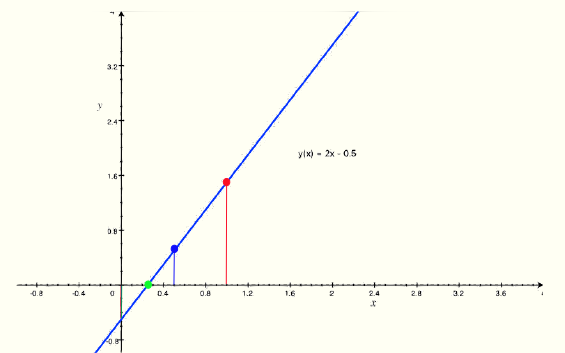
\includegraphics[width=.6\textwidth]{figures/plot}
	\end{figure}
When you are finished, post your code to the \textbf{Parabolic Interpolation Code} discussion board.	
\end{frame}

\end{document}
